
\chapter{SATELLITE ATTITUDE DYNAMICS AND KINEMATICS}
\label{chap:SatelliteAttitudeDynamicsAndKinematics}

This chapter covers the analytical modeling used in this research starting with the choice of attitude and body rate representations in Section \ref{sec:StateRepresentation}.  Next is a review of some of the estimation-based control methods used, including variations to target their use on spin-stabilized satellites such as NASA's MMS Mission spacecraft.

\section{Attitude Representation}
\label{sec:StateRepresentation}

The representation of the attitude of a spin-stabilized satellite is often accomplished using one of two representations: (1) Euler angles or (2) quaternions.  Quaternions are chosen for the attitude representation, as they provide unique advantages over Euler angles (te be expanded upon in Sections \ref{subsec:BodyRate} and \ref{subsec:QuaternionAttitude}.

\subsection{Angular Body Rates}
\label{subsec:BodyRate}

NASA's MMS satellites as with all real systems are rarely linear.  When modeling the dynamics of a system with nonlinearities, a common ``first pass'' is to linearize the model and assume that the nonlinearities are either negligible or can be lumped into a single system disturbances term.  This approach is also taken here.  The two portions of the system's dynamics are loosely generalized into either the rigid body dynamics of the satellite's main bus or the flexible dynamics of the attached flexible booms  Euler's Moment Equations are given as \cite{kaplan}:

\begin{subequations}
  \begin{align}
    M_x = \dot{h}_x + \omega_y h_z - \omega_z h_y \\
    M_y = \dot{h}_y + \omega_z h_x - \omega_x h_z \\
    M_z = \dot{h}_z + \omega_x h_y - \omega_y h_x
  \end{align}
  \label{eqn:EulerMoment}
\end{subequations}

where M represents the applied moment about the given axis and h and $\omega$ represent the corresponding angular momentum and velocity respectively.  Here the equations of motion are described in terms of the body's frame of reference ($x$, $y$, $z$) which does not necessarily align with the body's principal axes.  NASA MMS TableSat IA's construction can be simplified to an axisymmetric design.  To adjust TableSat's stability, the center screw can be raised or lowered bringing the center of mass and center of rotation closer or further apart.  As development of the observer-based controller improves, the two centers can be brought closer together.  With these conditions, we can assume that the body's reference frame aligns with the body's principal axes, which simplifies Euler's equations further to

\begin{subequations}
  \begin{align}
    M_x & = I_x \dot{\omega}_x + \omega_y \omega_z (I_z - I_y) \\
    M_y & = I_y \dot{\omega}_y + \omega_x \omega_z (I_x - I_z) \\
    M_z & = I_z \dot{\omega}_z + \omega_x \omega_y (I_y - I_x)
  \end{align}
  \label{eqn:EulerMomentPrincipleAxes}
\end{subequations}

For implementation into the TableSat's base station observer-based controller, the continuous time Euler's Equations in (\ref{eqn:EulerMomentPrincipleAxes}) are discretized with a variable time step and implemented (in Appendix \ref{code:TSatPy/State.py}) as

\begin{subequations}
  \begin{align}
    \dot{\omega}_{x}(t_{k}) & = \frac{1}{I_x} \left[ M_1(t_{k}) - (I_z - I_y) \omega_{y}(t_k) \omega_{z}(t_k) \right] \\
    \dot{\omega}_{y}(t_{k}) & = \frac{1}{I_y} \left[ M_2(t_{k}) - (I_x - I_z) \omega_{x}(t_k) \omega_{z}(t_k) \right] \\
    \dot{\omega}_{z}(t_{k}) & = \frac{1}{I_z} \left[ M_3(t_{k}) - (I_y - I_x) \omega_{x}(t_k) \omega_{y}(t_k) \right]
  \end{align}
  \label{eqn:DiscreteEulerMomentEquations}
\end{subequations}

Since the observer-based controller update frequencies are allowed to vary, the applied moment values may also have multiple values between times $t_{k}$ and $t_{k+1}$.  To simplify calculations, the value of the ``most recent'' moment is taken and assumed constant for $t$ such that $t_{k-1} < t < t_{k}$.  If the moment update loop is running slower than that of the Euler equation model, the last known moment is assumed to still be valid.

While the Euler equation model works well for propagating the system states only TableSat IA's attitude is measured leaving its body rates unmeasured.  A state observer/filter must then be used to estimate the unmeasured body rates.  In addition the observer/filter is also used to more accurately estimate attitude states. calculated through both observing changes in current attitude and state predictions based on previous attitude changes.  Euler angles and quaternions were investigated for parameterizing TableSat's attitude.

\subsection{Euler Angle Representation}

Euler angles were first considered for the attitude parameterization in this research because of their wide use in control theory where a body's attitude can be represented by a series of no more than three pure rotations: roll, pitch, and yaw.   There are twelve possible sequences.  The following shows the relationship between Euler angle rates and fixed-body angular velocities given a 3-1-3 rotation sequence \cite{kaplan}:

\begin{equation}
  \begin{bmatrix}
    \omega_x \\
    \omega_y \\
    \omega_z \\
  \end{bmatrix}
  =
  \begin{bmatrix}
    \sin \theta \sin \phi & \cos \phi & 0 \\
    \sin \theta \cos \phi & - \sin \phi & 0 \\
    \cos \theta & 0 & 1 \\
  \end{bmatrix}
  \begin{bmatrix}
    \dot{\psi} \\
    \dot{\theta} \\
    \dot{\phi} \\
  \end{bmatrix}
  \label{eqn:EulerToBodyRate}
\end{equation}

Here, $\psi, \theta,$ and $\phi$ represent Euler angles corresponding to the 3-1-3 rotation sequence.  Euler angles, while widely used and (for most people) easier to visualize, they have two main deficiencies.  They are heavily reliant on trigonometric functions and under certain conditions can cause singularities as seen by transforming Equation (\ref{eqn:EulerToBodyRate}) to solve for the Euler rates as seen in Equation (\ref{eqn:BodyRateToEuler}).  This phenomenon often results in gimbal lock.  The second deficiency occurs in implementation, where the efficiency and stability of the angles are tied to the accuracy of on-board trigonometric interpolations.  Repeated use of these approximations are prone to numerical drift.

\begin{equation}
  \begin{bmatrix}
    \dot{\psi} \\
    \dot{\theta} \\
    \dot{\phi} \\
  \end{bmatrix}
  =
  \frac{1}{\sin \theta}
  \begin{bmatrix}
    \sin \phi & \cos \phi & 0 \\
    \cos \phi \sin \theta & -\sin \phi \sin \theta & 0 \\
    -\sin \phi \cos \theta & -\cos \phi \cos \theta & \sin \theta \\
  \end{bmatrix}
  \begin{bmatrix}
    \omega_x \\
    \omega_y \\
    \omega_z \\
  \end{bmatrix}
  \label{eqn:BodyRateToEuler}
\end{equation}

The alternative attitude parameterization investigated is the quaternion attitude representation.  The relationship between discrete body rates and quaternion attitude via the method of Trawny and Roumeliotis \cite{marslab} is given as

\begin{equation}
  \bs{q}(t_{k+1}) = ( \bs{A} + \bs{B} ) \bs{q}(t_{k}) \\
  \label{eqn:DiscreteQuaternionPropagation}
\end{equation}
where
\begin{equation}
  \begin{aligned}
    \text{where } \bs{A} &= \exp \left( \frac{\Delta t_{k+1}}{2} \bs{\Omega} \left[ \bs{\bar{\omega}}(t_{k+1}) \right] \right)\\
    \bs{B} &= \frac{1}{48} \Delta t_{k+1}^2 \Big(
    \bs{\Omega} \left[\bs{\omega}(t_{k+1}) \right]
    \bs{\Omega} \left[\bs{\omega}(t_{k})   \right] -
    \bs{\Omega} \left[\bs{\omega}(t_{k})   \right]
    \bs{\Omega} \left[\bs{\omega}(t_{k+1}) \right]
      \Big)
  \end{aligned}
\end{equation}
\begin{equation}
    \bs{\Omega} \left[ \bs{\bar{\omega}}(t_{k+1}) \right] = \frac{\bs{\Omega} \left[\bs{\omega}(t_{k+1}) \right] + \bs{\Omega} \left[\bs{\omega}(t_{k}) \right]}{2}
    \label{eqn:DiscreteQuaternionToBodyRate}
\end{equation}
\begin{equation}
  \bs{\Omega} \left[ \bs{\omega} \right] =
  \begin{bmatrix}
    - [ \bs{\omega} \times ] & \bs{\omega} \\
    - \bs{\omega}^T & 0 \\
  \end{bmatrix}
  \label{eqn:OmegaMatrix}
\end{equation}
and where $\bs{\omega} \times$ is a skew-symmetric matrix defined as
\begin{equation}
  \bs{\omega} \times =
  \begin{bmatrix}
    0 & -\bs{\omega}_z & \bs{\omega}_y \\
    \bs{\omega}_z & 0 & -\bs{\omega}_x \\
    -\bs{\omega}_y & \bs{\omega}_x & 0 \\
  \end{bmatrix}
\end{equation}


\subsection{Quaternion Attitude Representation}
\label{subsec:QuaternionAttitude}

The concept of a quaternion is a combination of geometry and algebra from Rodrigues and Hamilton, respectively \cite{shuster}.  Rodrigues' work in the early 1800's focused the Gibbs vector as a way of creating a an attitude matrix from Rodrigues parameters.  Hamilton's work focused on hyper-complex numbers with three hyper-imaginary values and a constant.  Hamilton first coined the term quaternion in 1843 to describe the four dimensional vector.  The four orthogonal unit quaternions are

\begin{subequations}
  \begin{align}
    \bs{1} = & 1 + 0\bs{i} + 0\bs{j} + 0\bs{k} \\
    \bs{i} = & 0 + 1\bs{i} + 0\bs{j} + 0\bs{k} \\
    \bs{j} = & 0 + 0\bs{i} + 1\bs{j} + 0\bs{k} \\
    \bs{k} = & 0 + 0\bs{i} + 0\bs{j} + 1\bs{k}
  \end{align}
  \label{eqn:UnitQuaternions}
\end{subequations}
where the unit quaternions obey Hamilton's rules \cite{wolfram_quaternion}
\begin{subequations}
  \begin{align}
    \bs{i}^2 = \bs{j}^2 = \bs{k}^2 = \bs{ijk} & = - \bs{1} \\
    \bs{i}\bs{j} = -\bs{j}\bs{i} &= \bs{k} \\
    \bs{j}\bs{k} = -\bs{k}\bs{j} &= \bs{i} \\
    \bs{k}\bs{i} = -\bs{i}\bs{k} &= \bs{j}
  \end{align}
  \label{eqn:HamiltonRules}
\end{subequations}

As discussed in Section \ref{subsec:StateMeasurement}, between TableSat sensor and MMS Mission restrictions, the body rate for this research is not measured.  This means that the choice in attitude parameterization and how it is implemented significantly affects the system's overall performance.  Because of their numerical stability and the eventual intuitiveness of quaternions, the quaternion representation is chosen as the method for representing state attitude parameters in this research.  The quaternion notation to be used in this thesis follows the tensor structure where the scalar term follows the vector such that
\begin{equation}
  \bs{q} = \bs{v} + q_0 = q_1 \bs{i} + q_2 \bs{j} + q_3 \bs{k} + q_0
\end{equation}
where $\bs{v}$ is the vector portion of the quaternion and $q_0$ is the scalar term.

The ability to use a quaternion to represent a body's attitude is summarized by Euler's rotation theorem which states:

\begin{quote}{``\textsl{If $\bs{R}$ is a 3x3 orthogonal matrix $( \bs{R}^T \bs{R} = \bs{R}\bs{R}^T = \bs{I} )$ and $\bs{R}$ is proper $( det \bs{R} = +1 )$, then there is a nonzero vector $\bs{v}$ satisfying $\bs{Rv} = \bs{v}$}''~\cite{euler_theorem}}\end{quote}

With a 3x3 rotational matrix, this means there is a line of points that do not change position and create an axis of rotation.  Incorporating this idea into any spin-stabilized satellite like those in NASA's MMS Mission yields that any arbitrary attitude can be represented as a single rotation from a common starting orientation.  The Euler axis $\bs{\hat{e}}$ and the angle of rotation $\theta$ can express the satellite's attitude with a rotational quaternion as
\begin{equation}
  \bs{q} = \bs{v} + q_0 = \hat{\bs{e}} \sin \left( \frac{-\theta}{2} \right) + \cos \left( \frac{-\theta}{2} \right)
  \label{eqn:RotationalQuaternionDefinition}
\end{equation}
The negative $-\theta$ term is used instead of the standard positive value to allow visualizations to rotate points in the appropriate direction when viewed from the fixed inertial reference frame as some of the visualizations from Section \ref{sec:ObjectOrientedNSSControlSystem}.  Besides the quaternion definition in Equation (\ref{eqn:RotationalQuaternionDefinition}), the other key aspect of a rotational quaternion is that it maintains a unit norm as shown by calculating the norm of Equation (\ref{eqn:RotationalQuaternionDefinition})
\begin{equation}
  \left| \hat{\bs{e}} \sin \left( \frac{-\theta}{2} \right) + \cos \left( \frac{-\theta}{2} \right) \right| = \left| \hat{\bs{e}} \right|  \sin^2 \left( \frac{-\theta}{2} \right) + \cos^2 \left( \frac{-\theta}{2} \right) = 1
\end{equation}
This unit norm is a key property of rotational quaternions and is used in this research to assess the integrity of operations on quaternion states.

The quaternion multiplication, denoted with the infix operator $\otimes$, is the only method available to combine rotational quaternions and maintain the unit norm.  This quaternion multiplication is used to produce incremental changes in the satellite's attitude.  If $\bs{a}$ represents an $n$ degree rotation about axis $\hat{e}$, then a $4n$ degree rotation about axis $\bs{\hat{e}}$ can be represented as $\bs{a} \otimes \bs{a} \otimes \bs{a} \otimes \bs{a}$.

For example, let two quaternions $\bs{a}$ and $\bs{b}$ be represented as
\begin{subequations}
\begin{align}
  \bs{a} = \bs{a}_v + a_0 = & a_1 \bs{i} + a_2 \bs{j} + a_3 \bs{k} + a_0\\
  \bs{b} = \bs{b}_v + b_0 = & b_1 \bs{i} + b_2 \bs{j} + b_3 \bs{k} + b_0
\end{align}
\end{subequations}
The quaternion multiplication is defined as
\begin{equation}
  \bs{q} = \bs{a} \otimes \bs{b} = \bs{a}_v b_0 + \bs{b}_v a_0 + \bs{a}_v \times \bs{b}_v + a_0 b_0 - \bs{a}_v \cdot \bs{b}_v
  \label{eqn:QuaternionMultiplication}
\end{equation}
where $\bs{a}_v$, $a_0$, $\bs{b}_v$, and $b_0$ represent the vector and scalar components of the $\bs{a}$ and $\bs{b}$ quaternions respectively.  Expanding Equation (\ref{eqn:QuaternionMultiplication}) yields
\begin{subequations}
\begin{align}
  \bs{v} & = \begin{bmatrix} a_1 \\ a_2 \\ a_3 \end{bmatrix} b_0 +\begin{bmatrix} b_1 \\ b_2 \\ b_3 \end{bmatrix} a_0 + \begin{bmatrix} a_1 \\ a_2 \\ a_3 \end{bmatrix} \times \begin{bmatrix} b_1 \\ b_2 \\ b_3 \end{bmatrix} \\
  q_0 & = a_0 b_0 - \bs{a}_v \cdot \bs{b}_v
\end{align}
\end{subequations}
which in turn yields
\begin{subequations}
\begin{align}
  \bs{v} & = \begin{bmatrix} a_1 \\ a_2 \\ a_3 \end{bmatrix} b_0 +\begin{bmatrix} b_1 \\ b_2 \\ b_3 \end{bmatrix} a_0 + \begin{bmatrix} a_2b_3 - a_3b_2 \\ a_3b_1 - a_1b_3 \\ a_1b_2 - a_2b_1 \\ \end{bmatrix} \\
  q_0 & = a_0 b_0 - (a_1b_1 + a_2b_2 + a_3b_3)
\end{align}
\end{subequations}
and simplifies to
\begin{equation}
  \begin{bmatrix} \bs{v} \\ q_0 \end{bmatrix} =
  \begin{bmatrix}
    a_0 & - a_3 &   a_2 & a_1 \\
    a_3 &   a_0 & - a_1 & a_2 \\
  - a_2 &   a_1 &   a_0 & a_3 \\
  - a_1 & - a_2 & - a_3 & a_0
  \end{bmatrix}
  \begin{bmatrix}
  b_1 \\ b_2 \\ b_3 \\ b_0
  \end{bmatrix}
  \label{eqn:quat_mul_square_matrix}
\end{equation}
The resulting square matrix in Equation (\ref{eqn:quat_mul_square_matrix}) can be partitioned appropriately so that it can be expressed more compactly and in a way that conveys a better sense of how the quaternions interact during multiplication operations:
\begin{equation}
  \begin{bmatrix} \bs{v} \\ q_0 \end{bmatrix} =
  \begin{bmatrix}
    (\bs{a}_v \times) + \bs{I} a_0 & \bs{a}_v \\
    -\bs{a}_v^T                    & a_0 \\
  \end{bmatrix}
  \begin{bmatrix}
  \bs{b}_v \\ b_0
  \end{bmatrix}
  \label{eqn:QuaternionMultiplicationDerived}
\end{equation}

This quaternion class for TSatPy as will be covered in Chapter \ref{chap:TSatPy} allows for the a very close representation of Equation (\ref{eqn:QuaternionMultiplicationDerived}).

% The advantage to this notation is that is much easier to run in a Numerical Simulation Software (NSS like MATLAB or Octave) or other scripting language, but its layout is specific to our definition of the matrix where the scalar value follows the vector.  There is not clear consensus from the broader community on whether the vector or scalar should come first.  This can cause large issues when implementing a system using a externally provided library since both implementations expect a 4x4 matrix, and combining the logic from the two systems would require either rewriting of systems or spending extra cycles on the interface between the two systems converting the matrices from a scalar first to a scalar last layout and vice versa.

% The object oriented nature of the code written for this thesis reduces or eliminates the confusion.  When an instance of a quaternion class is created, the vector and scalar values are set as separate parameters on the object regardless of order.  So when used in computation the $\Re^3$ and $\Re^1$ values can be referenced directly through the vector and scalar properties respectively.  Chapter \ref{ch:object_oriented} will cover the structure of the code developed for the thesis in greater detail.  The specific code that governs interactions between quaternions in the model is in section \ref{code:lib/@quaternion/quaternion.m}.



\subsection{Quaternion Decomposition}
\label{subsec:QuaternionDecomposition}

For use in control systems, Section \ref{subsec:QuaternionDecompositionForNutationControl} cites the need for separating a quaternion into two quaternions.  One representing the rotational motion about the $z$-axis and the second describing the nutation about an axis in the $xy$ plane.  The attitude of TSat is represented by a single quaternion.  The change in attitude between two states can be modeled by the a rotation about a single axis.  Figure \ref{fig:PreDecomposedQuaternion} show the attitude of a system described by the quaternion $\bs{q} = [\alpha, \beta, \phi], 0.16953$ which is a rotation of 2.8 radians about the axis $[\alpha, \beta, \phi]^T$.  For control purposes, decomposing the single quaternion into one representing a rotation about the z-axis and a second rotation about an axis in the x-y plane as shown in Figure \ref{fig:PostDecomposedQuaternion}.

\begin{figure}[H]
  \begin{subfigure}[h!]{0.5\textwidth}
    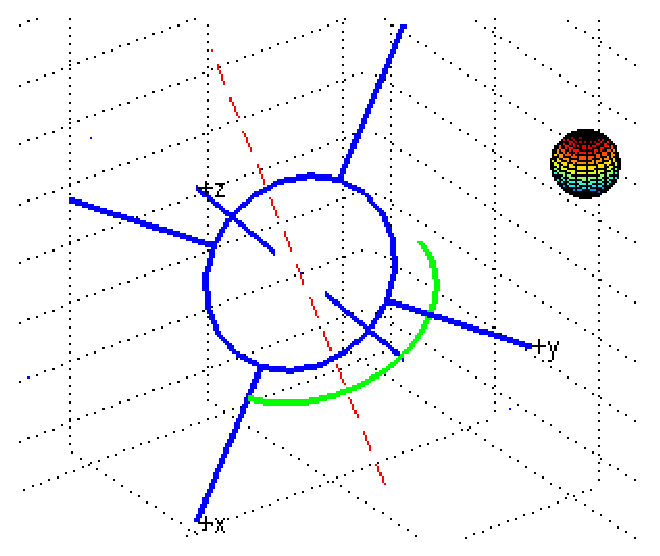
\includegraphics[width=\textwidth]{figures/quaternion_decompose_pre.eps}
    \caption{Quaternion State}
    \label{fig:PreDecomposedQuaternion}
  \end{subfigure}
  ~
  \begin{subfigure}[h!]{0.5\textwidth}
    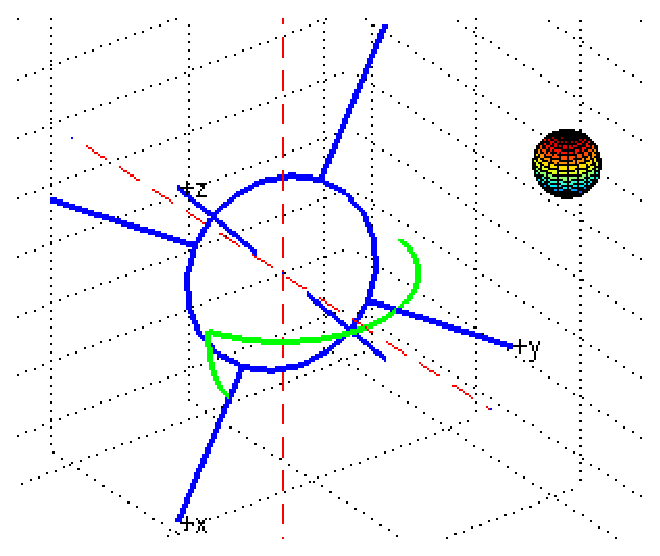
\includegraphics[width=\textwidth]{figures/quaternion_decompose_post.eps}
    \caption{Decomposed State}
    \label{fig:PostDecomposedQuaternion}
  \end{subfigure}
  \caption{Decomposing a Quaternion into Rotation and Nutation}
  \label{fig:QuaternionDecomposition}
\end{figure}

The quaternion that describes TSat's attitude $\bs{q}$ can be written as a sequence of two rotations.  A quaternion rotation about the z-axis $\bs{q_r}$ followed by the quaternion rotation about an axis in the x-y plane that creates a nutation $\bs{q_n}$.  Resultant rotations are performed through a left quaternion multiplication.
\begin{equation}
  \bs{q} = \bs{q_n} \otimes \bs{q_r} = \begin{bmatrix} \bs{v}_n \\ q_{0n} \end{bmatrix} \otimes \begin{bmatrix} \bs{v}_r \\ q_{0r} \end{bmatrix}
\end{equation}
\begin{equation}
  \begin{bmatrix}\bs{v} \\ q_{0} \end{bmatrix} =
  \begin{bmatrix} \bs{v}_n q_{0r} + \bs{v}_r q_{0n} + \bs{v}_n \times \bs{v}_r \\  q_{0n} q_{0r} - \bs{v}_n \cdot \bs{v}_r \end{bmatrix}
  \label{eqn:rot_nut_product}
\end{equation}
Expanding the vector components out creates the equation.
\begin{equation}
  \begin{bmatrix}
    q_{1} \\
    q_{2} \\
    q_{3} \\
    q_{0}
  \end{bmatrix}
  =
  \begin{bmatrix}
    \begin{bmatrix}
      q_{1n} \\
      q_{2n} \\
      q_{3n} \\
    \end{bmatrix} q_{0r} + \begin{bmatrix}
      q_{1r} \\
      q_{2r} \\
      q_{3r} \\
    \end{bmatrix} q_{0n} + \begin{bmatrix}
      q_{1n} \\
      q_{2n} \\
      q_{3n} \\
    \end{bmatrix} \times \begin{bmatrix}
      q_{1r} \\
      q_{2r} \\
      q_{3r} \\
    \end{bmatrix}
    \\
    q_{0n} q_{0r} - \begin{bmatrix}
      q_{1n} \\
      q_{2n} \\
      q_{3n} \\
    \end{bmatrix} \cdot \begin{bmatrix}
      q_{1r} \\
      q_{2r} \\
      q_{3r} \\
    \end{bmatrix} \\
  \end{bmatrix}
\end{equation}
and through simplification becomes
\begin{equation}
  \begin{bmatrix}
    q_{1} \\
    q_{2} \\
    q_{3} \\
    q_{0}
  \end{bmatrix}
  =
  \begin{bmatrix}
    q_{1n} q_{0r} + q_{1r} q_{0n} + q_{2n} q_{3r} - q_{3n} q_{2r} \\
    q_{2n} q_{0r} + q_{2r} q_{0n} + q_{3n} q_{1r} - q_{1n} q_{3r} \\
    q_{3n} q_{0r} + q_{3r} q_{0n} + q_{1n} q_{2r} - q_{2n} q_{1r} \\
  q_{0n} q_{0r} - (q_{1n} q_{1r} + q_{2n} q_{2r} + q_{3n} q_{3r} ) \\
  \end{bmatrix}
  \label{eqn:rot_nut_product_simplified}
\end{equation}
Now that we have an expanded representation of the resultant quaternion, we can use the restriction from the desired spin-stabilized state for TableSat.  The rotational quaternion is allowed to move freely about the $z$-axis but should not have any displacement about the $x$ and $y$ axes.  From Equation (\ref{eqn:RotationalQuaternionDefinition}), $q_{1r} = q_{2r} = 0$.
\begin{equation}
  \bs{q_{r}}
  = q_{1r} \bs{i} + q_{2r} \bs{j} + q_{3r} \bs{k} + q_{0r}
  = 0 \bs{i} + 0 \bs{j} + q_{3r} \bs{k} + q_{0r}
  \label{eqn:rotation_quaternion_defined}
\end{equation}
The nutation quaternion has the opposite restrictions where rotation is allowed about the $x$ and $y$ axes but not about the $z$ axis.  From Equation (\ref{eqn:RotationalQuaternionDefinition}), $q_{3n} = 0$.
\begin{equation}
  \bs{q_{n}}
  = q_{1n} \bs{i} + q_{2n} \bs{j} + q_{3n} \bs{k} + q_{0n}
  = q_{1n} \bs{i} + q_{2n} \bs{j} + 0 \bs{k} + q_{0n}
  \label{eqn:nutation_quaternion_defined}
\end{equation}
Substituting equations \eqref{eqn:rotation_quaternion_defined} and \eqref{eqn:nutation_quaternion_defined} into \eqref{eqn:rot_nut_product_simplified} yields.
\begin{equation}
  \begin{bmatrix}
    q_{1} \\
    q_{2} \\
    q_{3} \\
    q_{0}
  \end{bmatrix}
  =
  \begin{bmatrix}
    q_{1n} q_{0r} + 0             + q_{2n} q_{3r} - 0 \\
    q_{2n} q_{0r} + 0             + 0             - q_{1n} q_{3r} \\
    0             + q_{3r} q_{0n} + 0             - 0 \\
  q_{0n} q_{0r} - (q_{1n} 0 + q_{2n} 0 + 0 q_{3r} ) \\
  \end{bmatrix}
\end{equation}
\begin{subequations}
  \begin{align}
    q_{1} &= q_{1n} q_{0r} + q_{2n} q_{3r} \label{eqn:rot_nut_1_1} \\
    q_{2} &= q_{2n} q_{0r} - q_{1n} q_{3r} \label{eqn:rot_nut_1_2} \\
    q_{3} &= q_{3r} q_{0n} \label{eqn:rot_nut_1_3} \\
    q_{0} &= q_{0n} q_{0r} \label{eqn:rot_nut_1_0}
  \end{align}
\end{subequations}
Solving \ref{eqn:rot_nut_1_3} and \ref{eqn:rot_nut_1_0} for $q_{3r}$ and $q_{0r}$ and substituting into \ref{eqn:rot_nut_1_1} and \ref{eqn:rot_nut_1_2}
\begin{subequations}
  \begin{align}
    q_{0n} q_{1} &= q_{1n} q_{0} + q_{2n} q_{3} \label{eqn:rot_nut_2_1} \\
    q_{0n} q_{2} &= q_{2n} q_{0} - q_{1n} q_{3} \label{eqn:rot_nut_2_2}
  \end{align}
\end{subequations}
combining \ref{eqn:rot_nut_2_1} and \ref{eqn:rot_nut_2_2}
\begin{equation}
  0 = (q_{0}q_{2} + q_{1}q_{3}) q_{1n} + (q_{2}q_{3} - q_{0}q_{1}) q_{2n}
\end{equation}
\begin{subequations}
  \begin{align}
    q_{1n} &= Q \cdot q_{2n} \\
    \text{where } Q &= \frac{q_{0}q_{1} - q_{2}q_{3}}{q_{0}q_{2} + q_{1}q_{3}}
  \end{align}
  \label{eqn:nutation_parameter_ratio}
\end{subequations}
The additional restriction than rotational quaternions have a unit norm can be leveraged in finding solutions
\begin{equation}
  \left\| \bs{q} \right\| = \sqrt{\bs{v} \cdot \bs{v} + q_0^2} = \sqrt{q_1^2+q_2^2+q_3^2+q_0^2}
  \label{eqn:quaternion_norm}
\end{equation}
Taking the norm of the rotational quaternion in Equation (\ref{eqn:rotation_quaternion_defined}) and substituting $q_{3r}$ and $q_{0r}$ from Equations \ref{eqn:rot_nut_1_3} and \ref{eqn:rot_nut_1_0} becomes
\begin{equation}
  (0)^2 + (0)^2 + \left( \frac{q_3}{q_{0n}} \right)^2 + \left( \frac{q_0}{q_{0n}} \right)^2 = 1
\end{equation}
solving for $q_{n0}$
\begin{equation}
  q_{n0} = \pm \sqrt{q_3^2 + q_0^2}
  \label{eqn:nutation_scalar}
\end{equation}
substituting \ref{eqn:nutation_parameter_ratio} and \ref{eqn:nutation_scalar} into \ref{eqn:nutation_quaternion_defined}
\begin{equation}
  \bs{q_{n}}
  = Q \cdot q_{2n} \bs{i} + q_{2n} \bs{j} + 0 \bs{k} \pm \sqrt{q_3^2 + q_0^2}
\end{equation}
and as this is a rotational quaternion, its norm should always equal one
\begin{equation}
  (Q \cdot q_{2n})^2 + (q_{2n})^2 + (q_3^2 + q_0^2) = 1
\end{equation}
which can be solved for the nutation quaternion's $q_{2n}$ term
\begin{equation}
  q_{2n} = \pm \sqrt{ \frac{1  - q_3^2 - q_0^2}{Q^2 + 1} }
  \label{eqn:qn2_solution}
\end{equation}

We now have a mapping of the original state quaternion $\bs{q}$ to its decomposed rotation $\bs{q}_r$ and nutation $\bs{q}_n$ quaternions (Equation (\ref{eqn:quaternion_decomposition_derivation})).  The ability to break the attitude parameters into these two quantities is particularly useful for spin-stabilized satellites as it decouples the rate and attitude controllers.  Normally the attitude controller would need to propagate the desired quaternion attitude with input from the body rates. In this approach, the controller can ignore continuously changing rotational component $\bs{q}_r$, and limit its focus on driving the nutation error $\bs{q}_n$ to zero (Figure \ref{fig:PostDecomposedQuaternion}).
\begin{equation}
  \begin{aligned}
    \bs{q} &= \bs{q_n} \otimes \bs{q_r} \\
    \text{where } \bs{q}_n &= \begin{bmatrix} q_{1n} = Q \cdot q_{2n} \\ q_{2n} = \sqrt{ \frac{1  - q_3^2 - q_0^2}{Q^2 + 1} } \\ 0 \\ q_{0n} = \sqrt{q_3^2 + q_0^2} \end{bmatrix} , \bs{q}_r = \begin{bmatrix} 0 \\ 0 \\ q_{3r} = \frac{q_3}{q_{0n}} \\ q_{0r} = \frac{q_0}{q_{0n}} \end{bmatrix} \\
    Q &= \frac{q_{0}q_{1} - q_{2}q_{3}}{q_{0}q_{2} + q_{1}q_{3}}
  \end{aligned}
  \label{eqn:quaternion_decomposition_derivation}
\end{equation}
